\sectionframe{Background of my Masters Thesis}
\section{Background}

\begin{frame}{Continuous Model}
	\vspace{-1em}
	\begin{columns}
		\begin{column}{.4 \textwidth}
			\begin{itemize}
				\item DC/AC power converter
				\item Variable switching
			\end{itemize}
		\end{column}
		\begin{column}{.6 \textwidth}
			\begin{figure}
				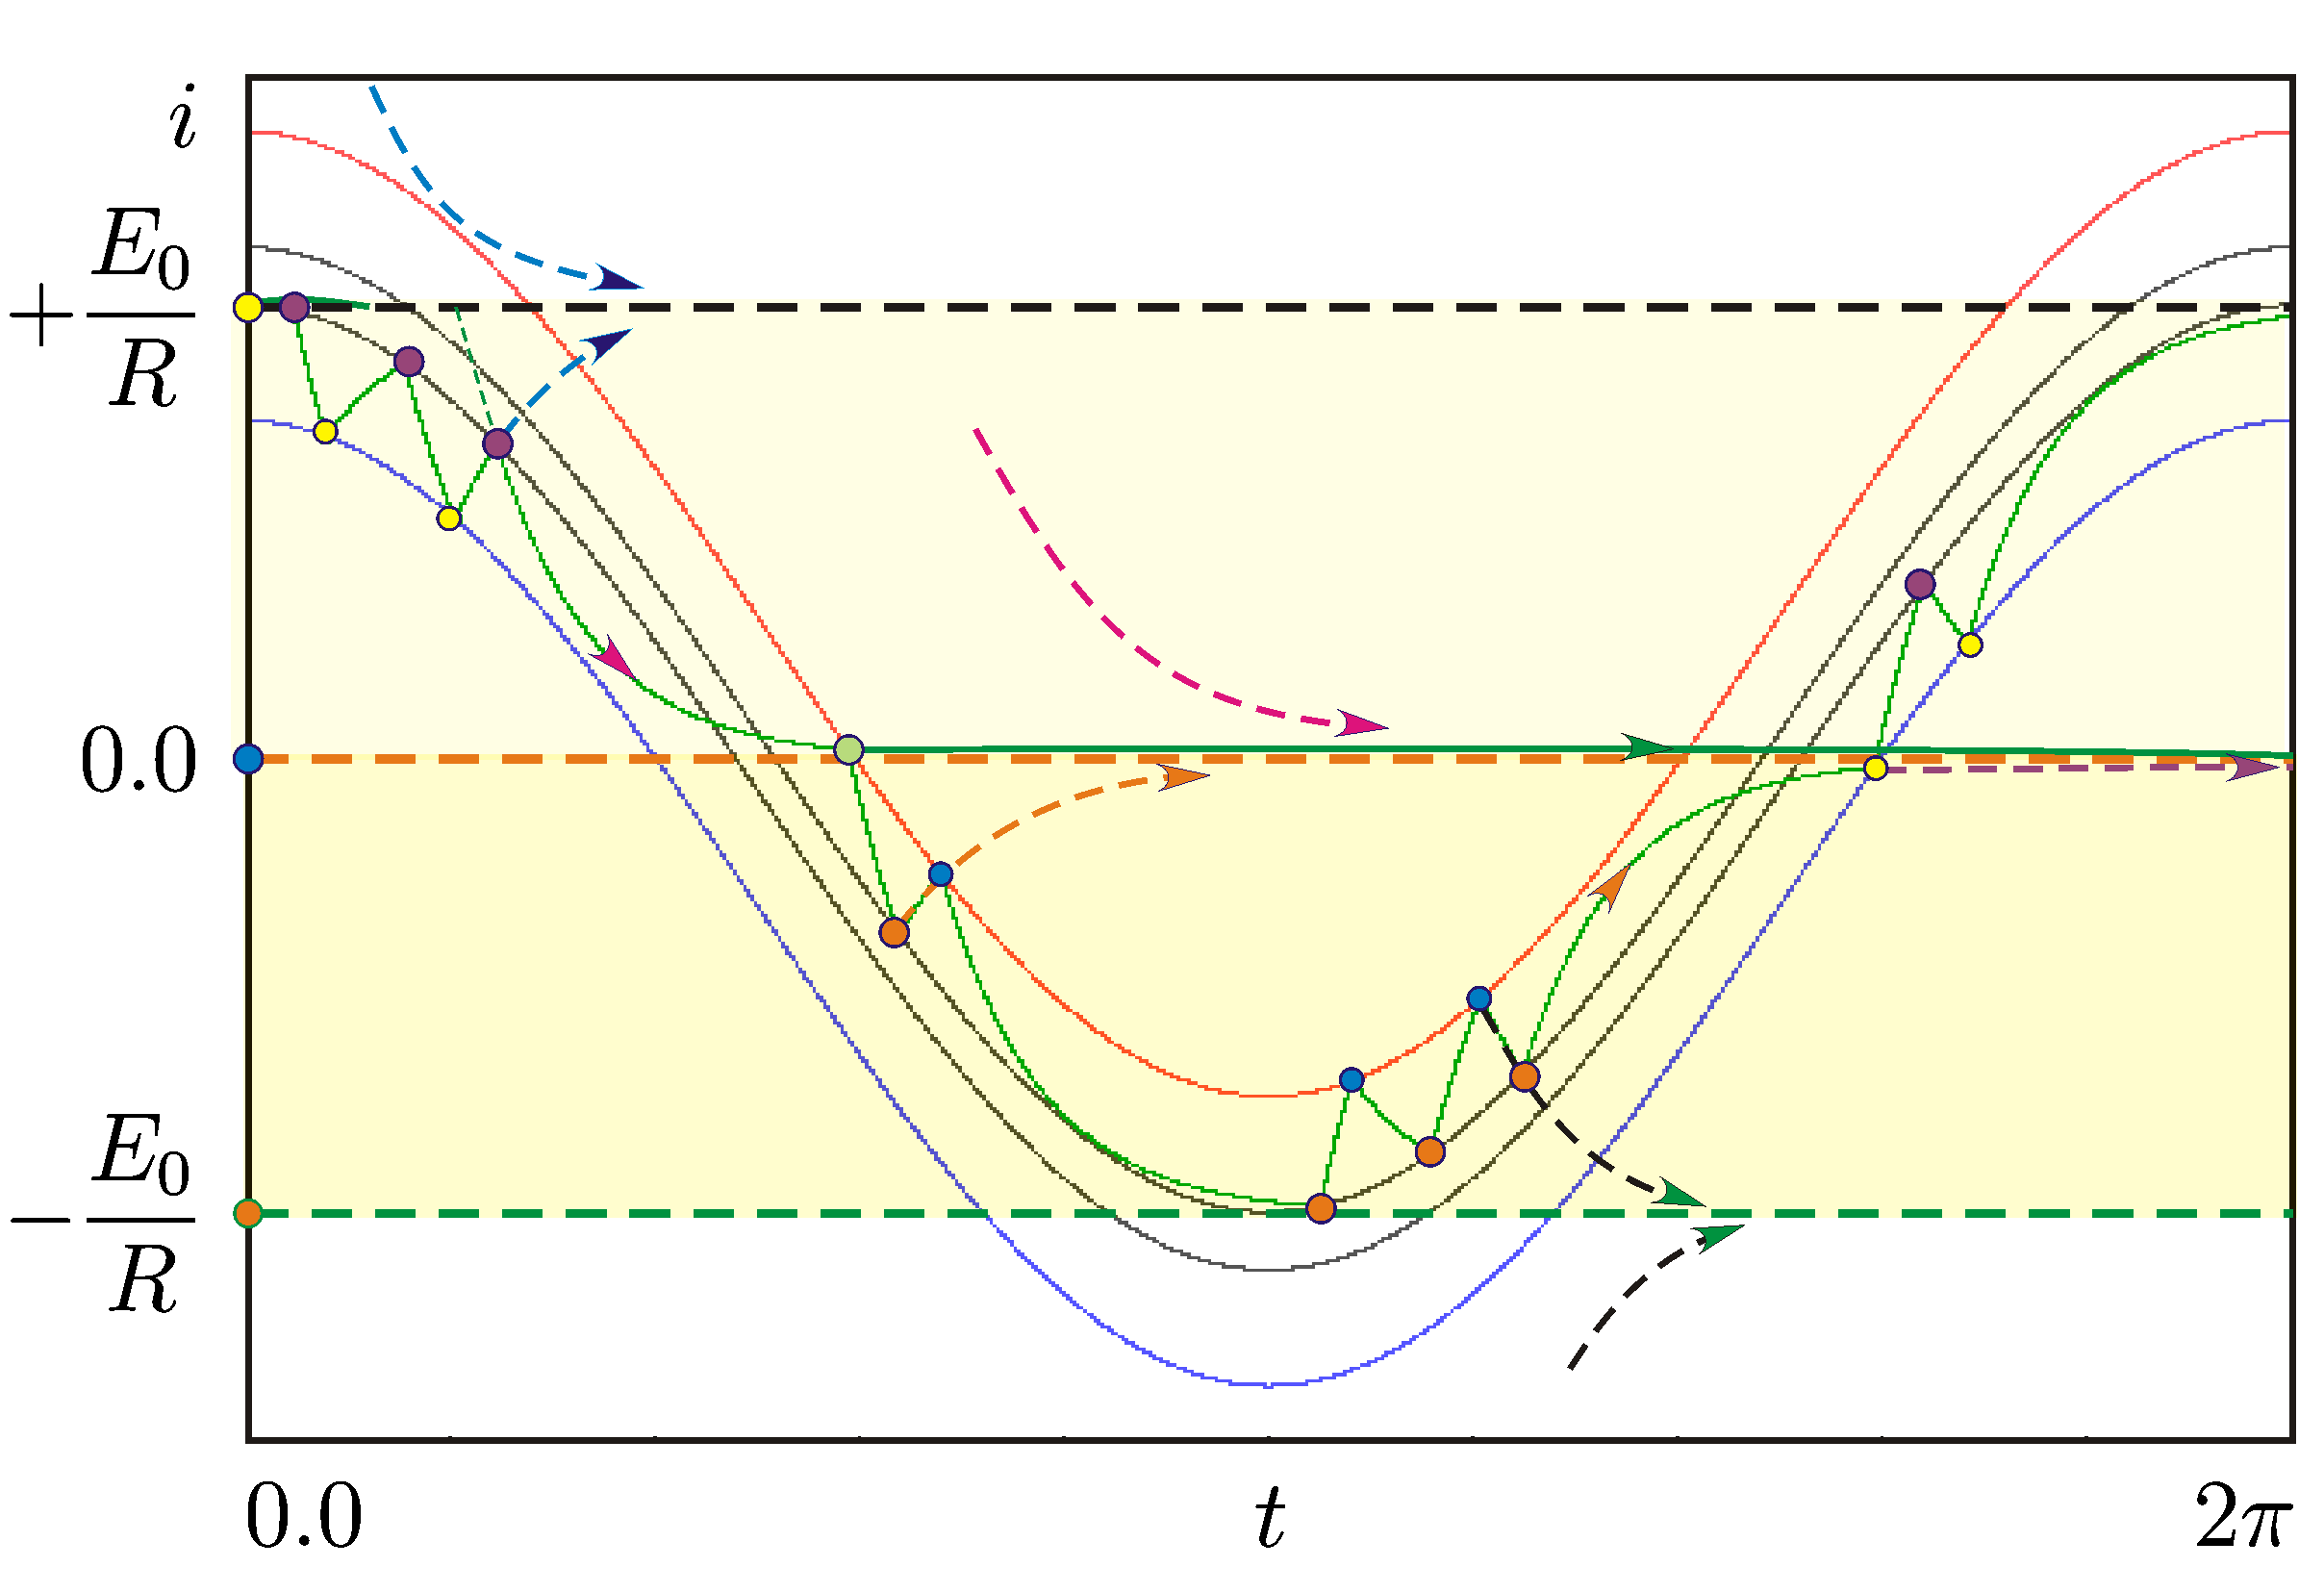
\includegraphics[width=0.8 \textwidth]{Figs/continuous_model.png}
			\end{figure}

			\flushright{[Zhusubaliyev]}
		\end{column}
	\end{columns}
\end{frame}

\begin{frame}{Discrete Model}
	\only<1>{
		\vspace{-2em}
		\begin{align*}
			\theta_{n+1} & =  F(\theta_n) \mod 2 \pi
			\\
			F(\theta)    & = \begin{cases}
				                 F_1(\theta) & \text{if } q \cdot \cos(\theta) > 0 \\
				                 F_2(\theta) & \text{if } q \cdot \cos(\theta) < 0
			                 \end{cases}
			\\
			F_1(\theta)  & = \begin{cases}
				                 \theta + z^{+} + z_{1}^{+}     & \text{if } z^{+} < z_{0}^{+} \\
				                 \theta + z_{0}^{+} + z_{2}^{+} & \text{if } z^{+} > z_{0}^{+}
			                 \end{cases}
			\\
			F_2(\theta)  & = \begin{cases}
				                 \theta + z^{-} + z_{1}^{-}     & \text{if } z^{-} < z_{0}^{-} \\
				                 \theta + z_{0}^{-} + z_{2}^{-} & \text{if } z^{-} > z_{0}^{-}
			                 \end{cases}
		\end{align*}

		\vspace{1em}
		Values of $ z^{+}, z_{1}^{+}, z_{0}^{+}, z_{2}^{+}, z^{-}, z_{1}^{-}, z_{0}^{-}, \text{ and } z_{2}^{-}$?
	}
	\only<2>{
		\vspace{-3em}
		\begin{align*}
			(q \cdot \cos(\theta) - \chi_{c}) \cdot e^{\lambda \cdot z^{+}}
			 & = q \cdot \cos(\theta + z^{+}) - \chi_{0}                  \\
			(q \cdot \cos(\theta + z^{+}) - \chi_{0} - 1) \cdot e^{\lambda \cdot z_{1}^{+}} + 1
			 & = q \cdot  \cos(\theta + z^{+} + z_{1}^{+}) - \chi_{c}     \\
			(q \cdot \cos(\theta) - \chi_{c}) \cdot e^{\lambda \cdot z_{0}^{+}}
			 & = q \cdot \cos(\theta + z_{0}^{+}) + \chi_{0}              \\
			(q \cdot \cos(\theta + z_{0}^{+} + z_{2}^{+}) + \chi_{0} + 1) \cdot e^{\lambda \cdot z_{2}^{+}} - 1
			 & = q \cdot  \cos(\theta + z_{0}^{+} + z_{2}^{+}) + \chi_{c} \\[1em]
			(q \cdot \cos(\theta) + \chi_{c}) \cdot e^{\lambda \cdot z^{-}}
			 & = q \cdot \cos(\theta + z^{-}) + \chi_{0}                  \\
			(q \cdot \cos(\theta + z^{-}) + \chi_{0} + 1) \cdot e^{\lambda \cdot z_{1}^{-}} - 1
			 & = q \cdot  \cos(\theta + z^{-} + z_{1}^{-}) + \chi_{c}     \\
			(q \cdot \cos(\theta) + \chi_{c}) \cdot e^{\lambda \cdot z_{0}^{-}}
			 & = q \cdot \cos(\theta + z_{0}^{-}) - \chi_{0}              \\
			(q \cdot \cos(\theta + z_{0}^{-} + z_{2}^{-}) - \chi_{0} - 1) \cdot e^{\lambda \cdot z_{2}^{-}} + 1
			 & = q \cdot  \cos(\theta + z_{0}^{-} + z_{2}^{-}) - \chi_{c} \\
		\end{align*}
		\vspace{-3em}
		\begin{flushright}
			Smallest positive solutions
			\hfill
			[Akyuz, Avrutin]
		\end{flushright}
	}
\end{frame}

\begin{frame}{Unusual Bifurcation Structure}
	\only<1>{
		\begin{figure}
			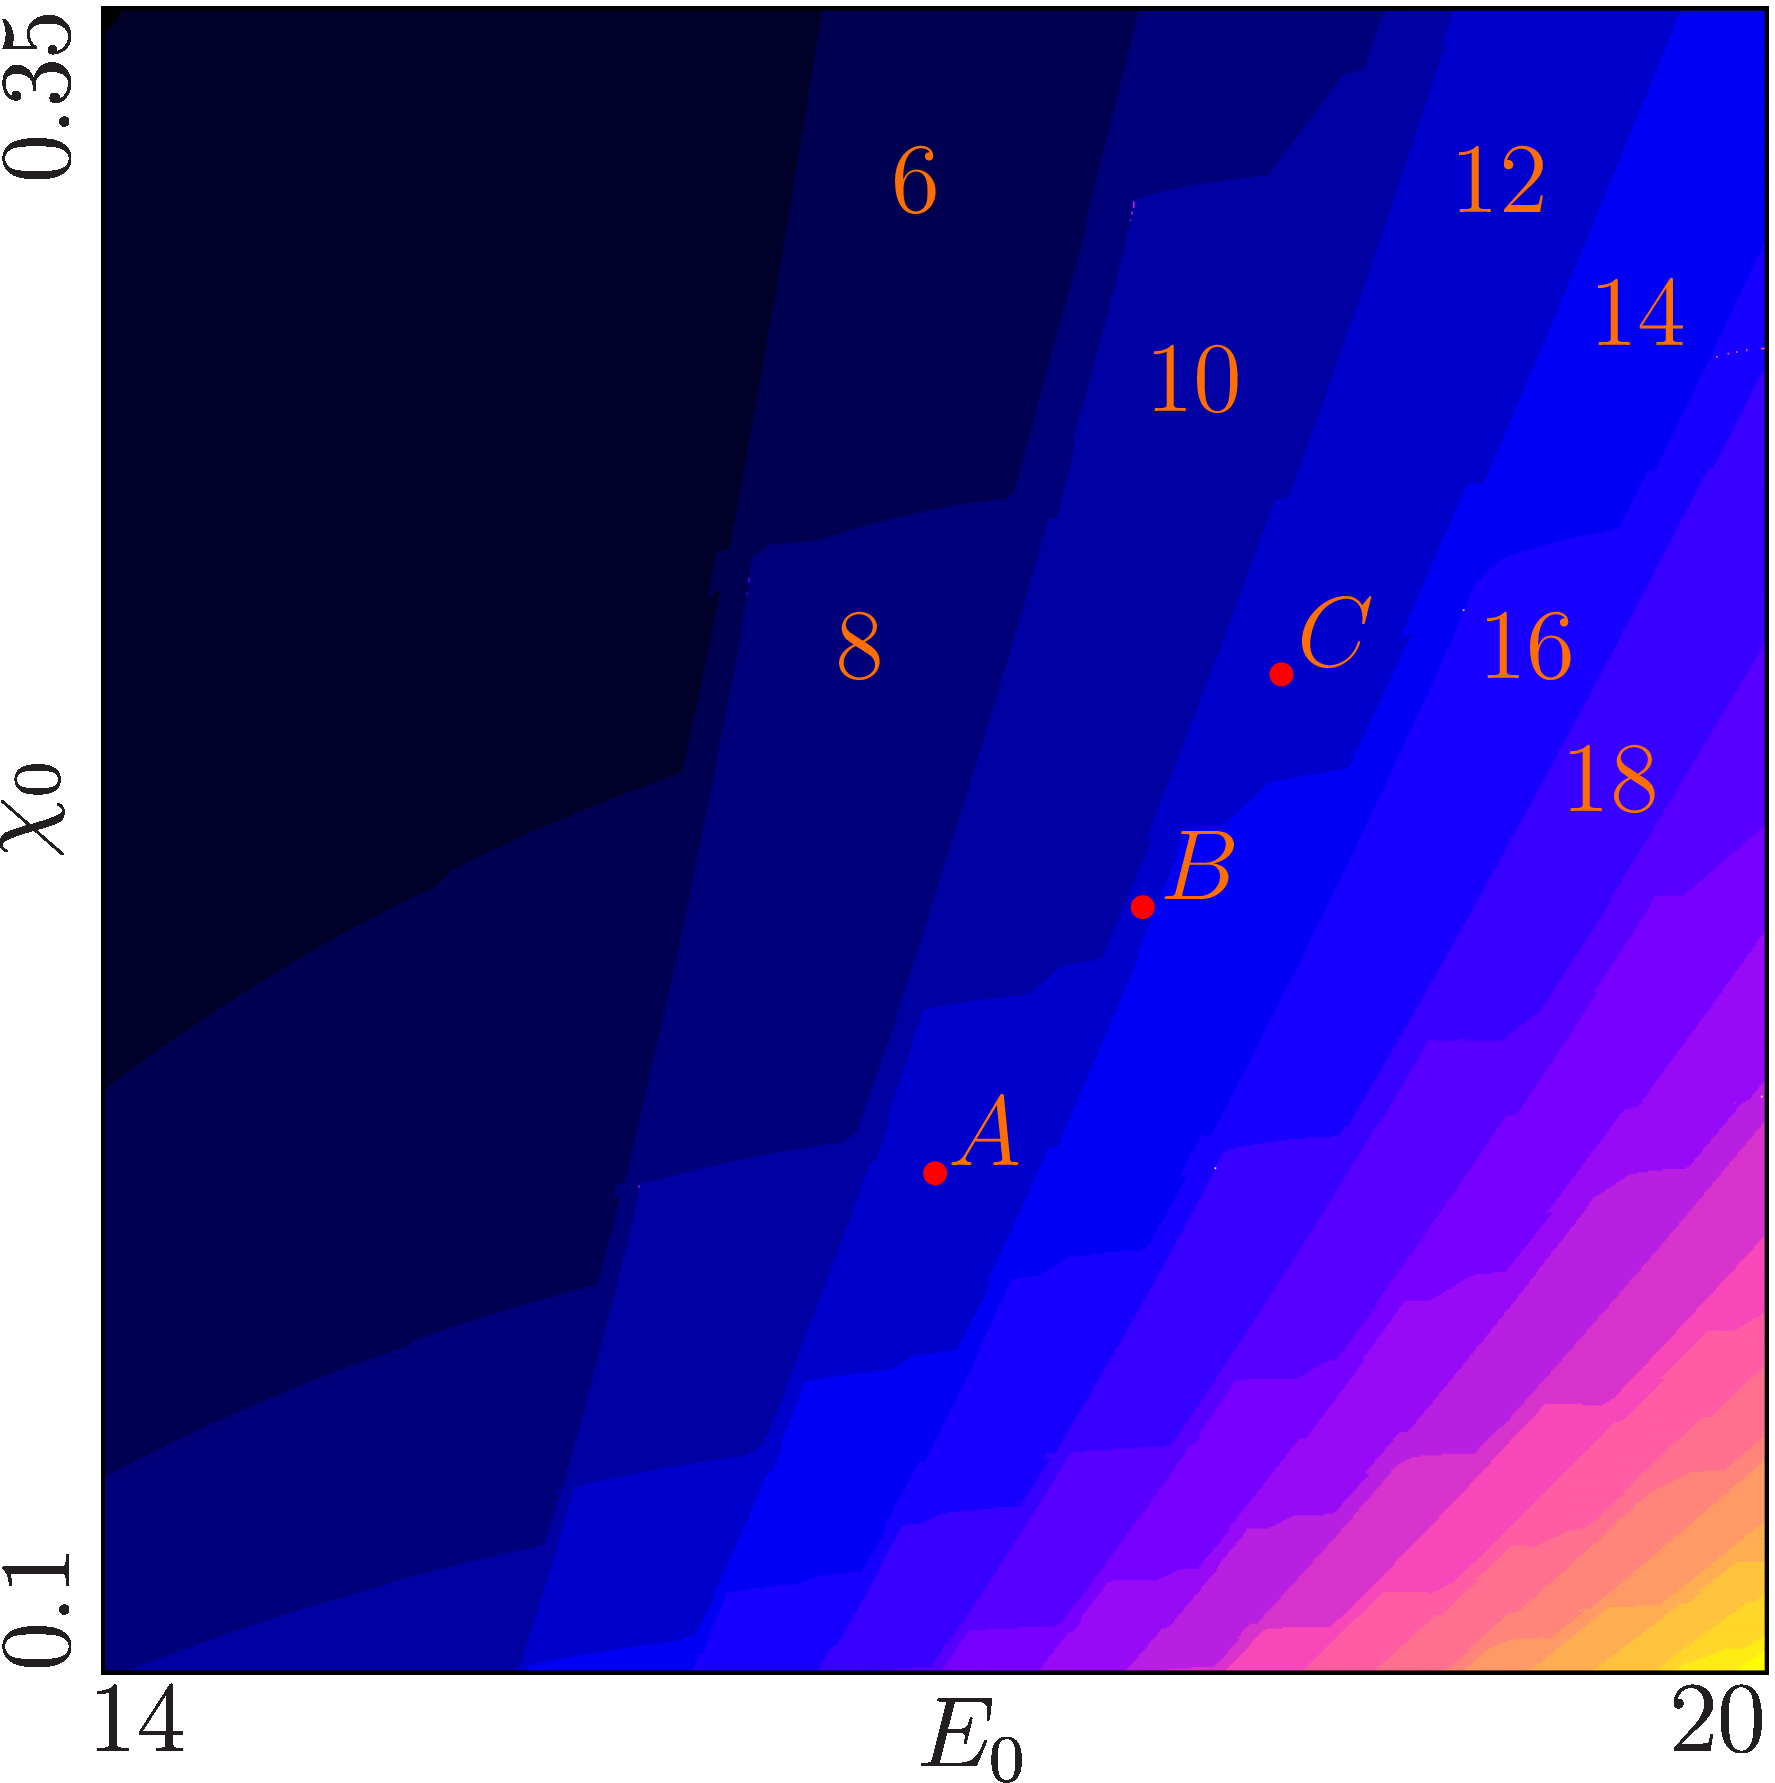
\includegraphics[width=0.45 \textwidth]{Figs/og_model_period.png}
		\end{figure}
	}
	\only<2>{
		\begin{figure}
			\stackunder[5pt]{
				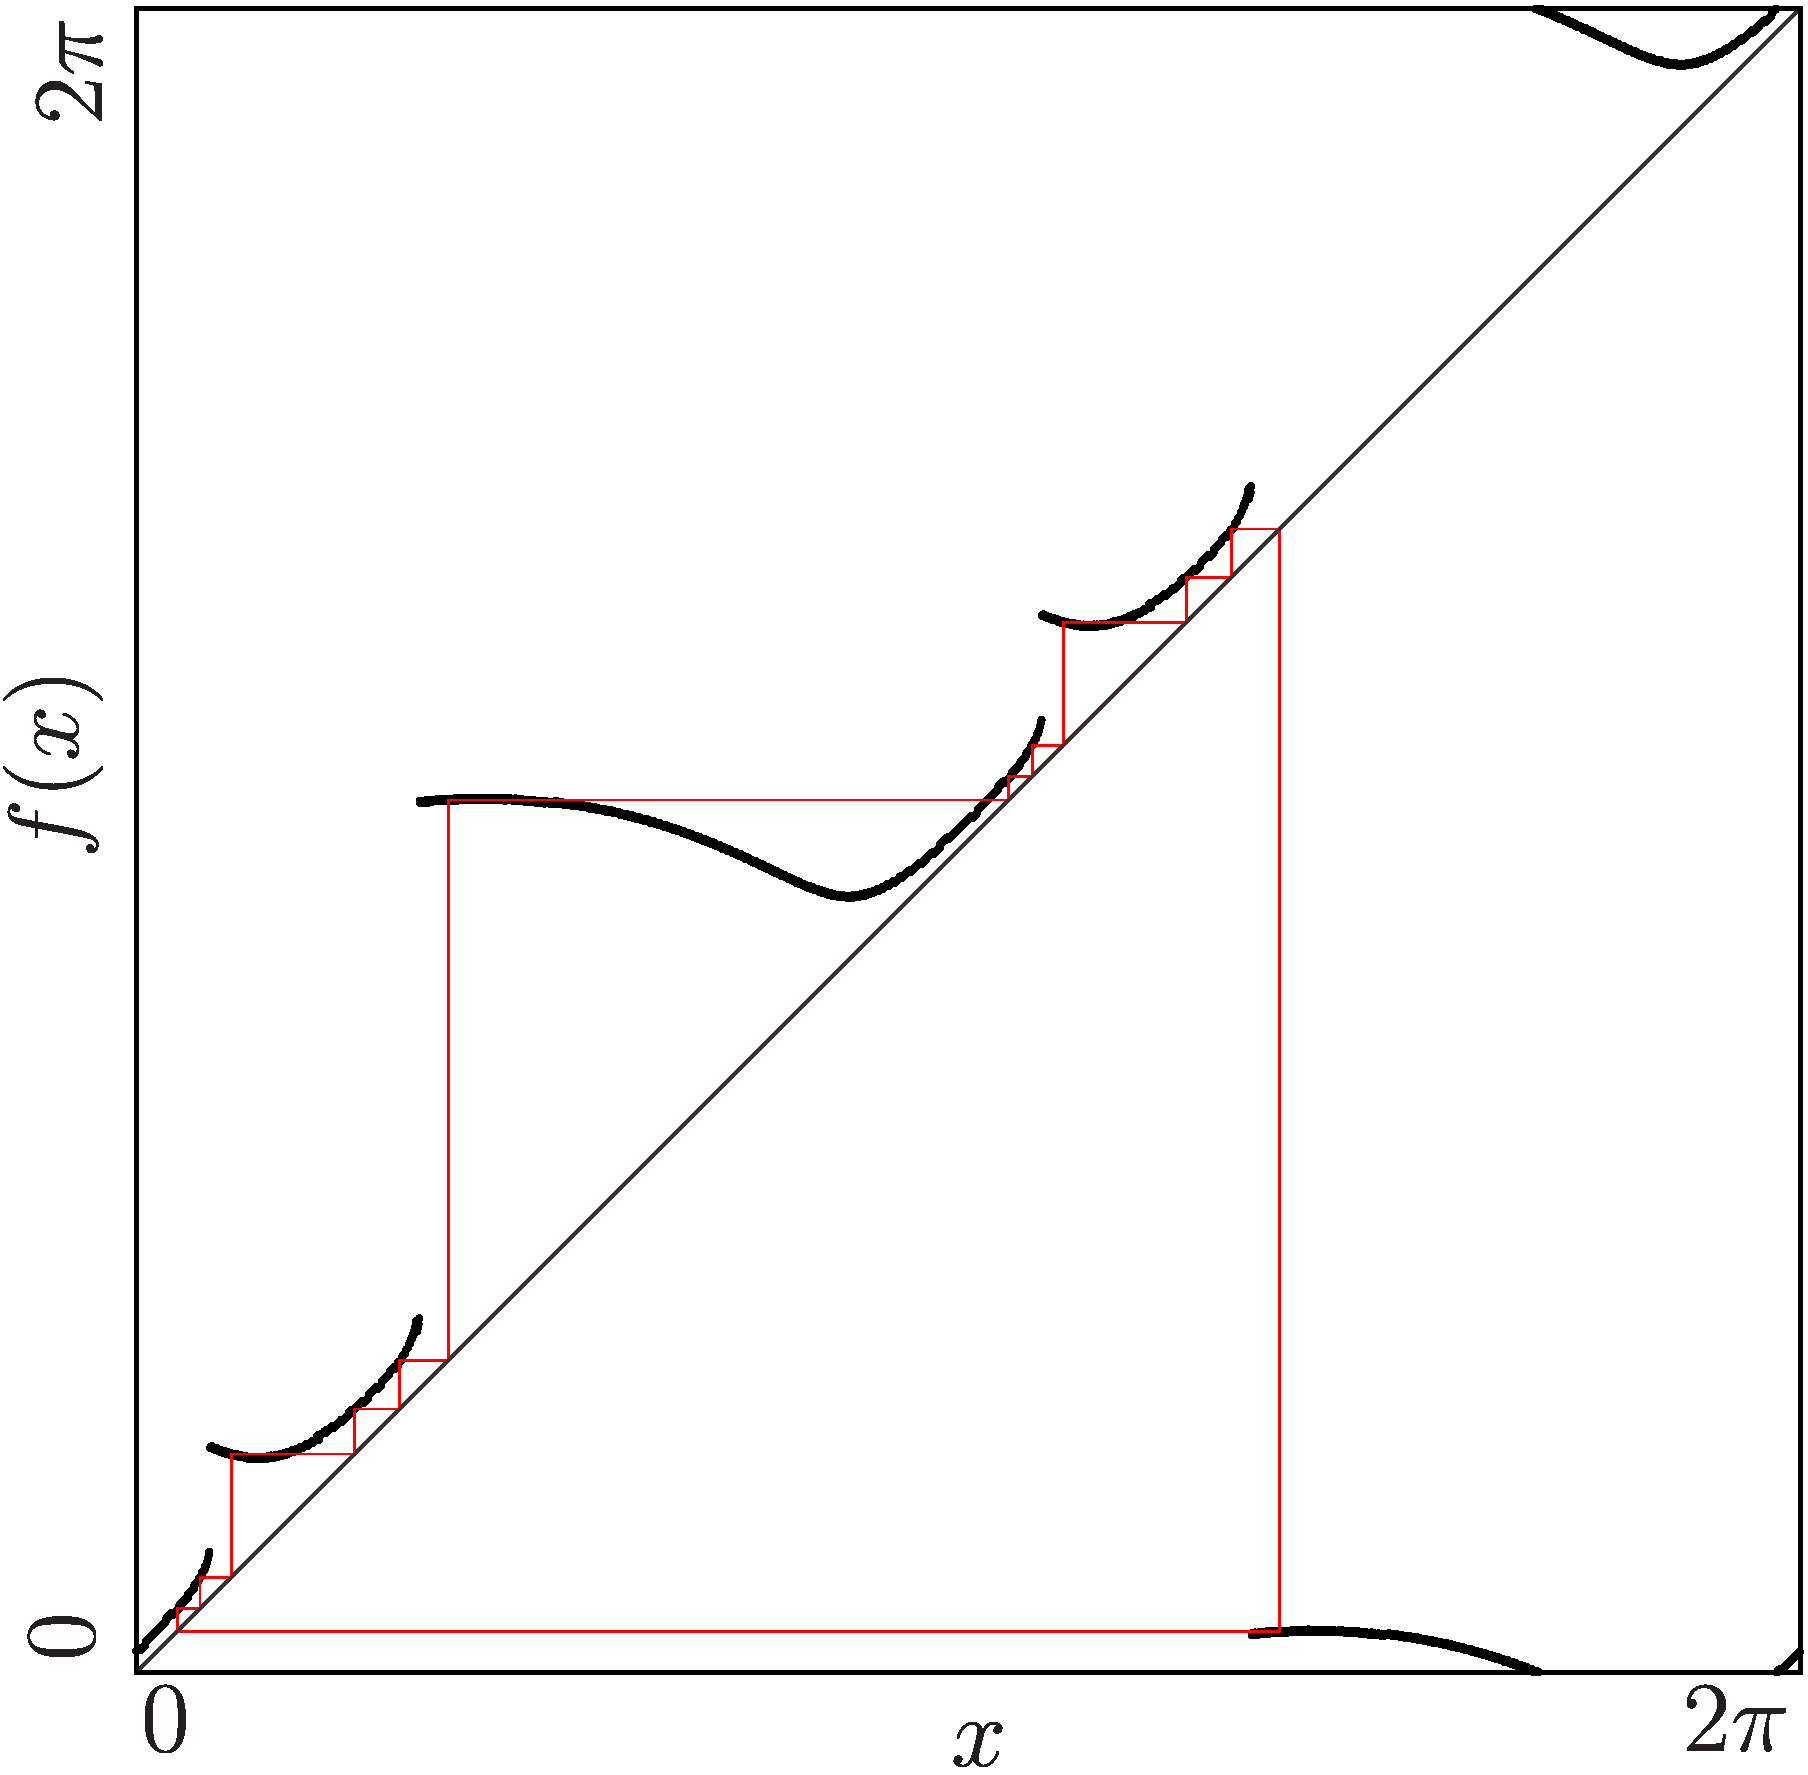
\includegraphics[width=0.3 \textwidth]{Figs/og_model_cycle_a.png}
			}{$A:\:\A^3\B^3\C^3\D^3$}
			\stackunder[5pt]{
				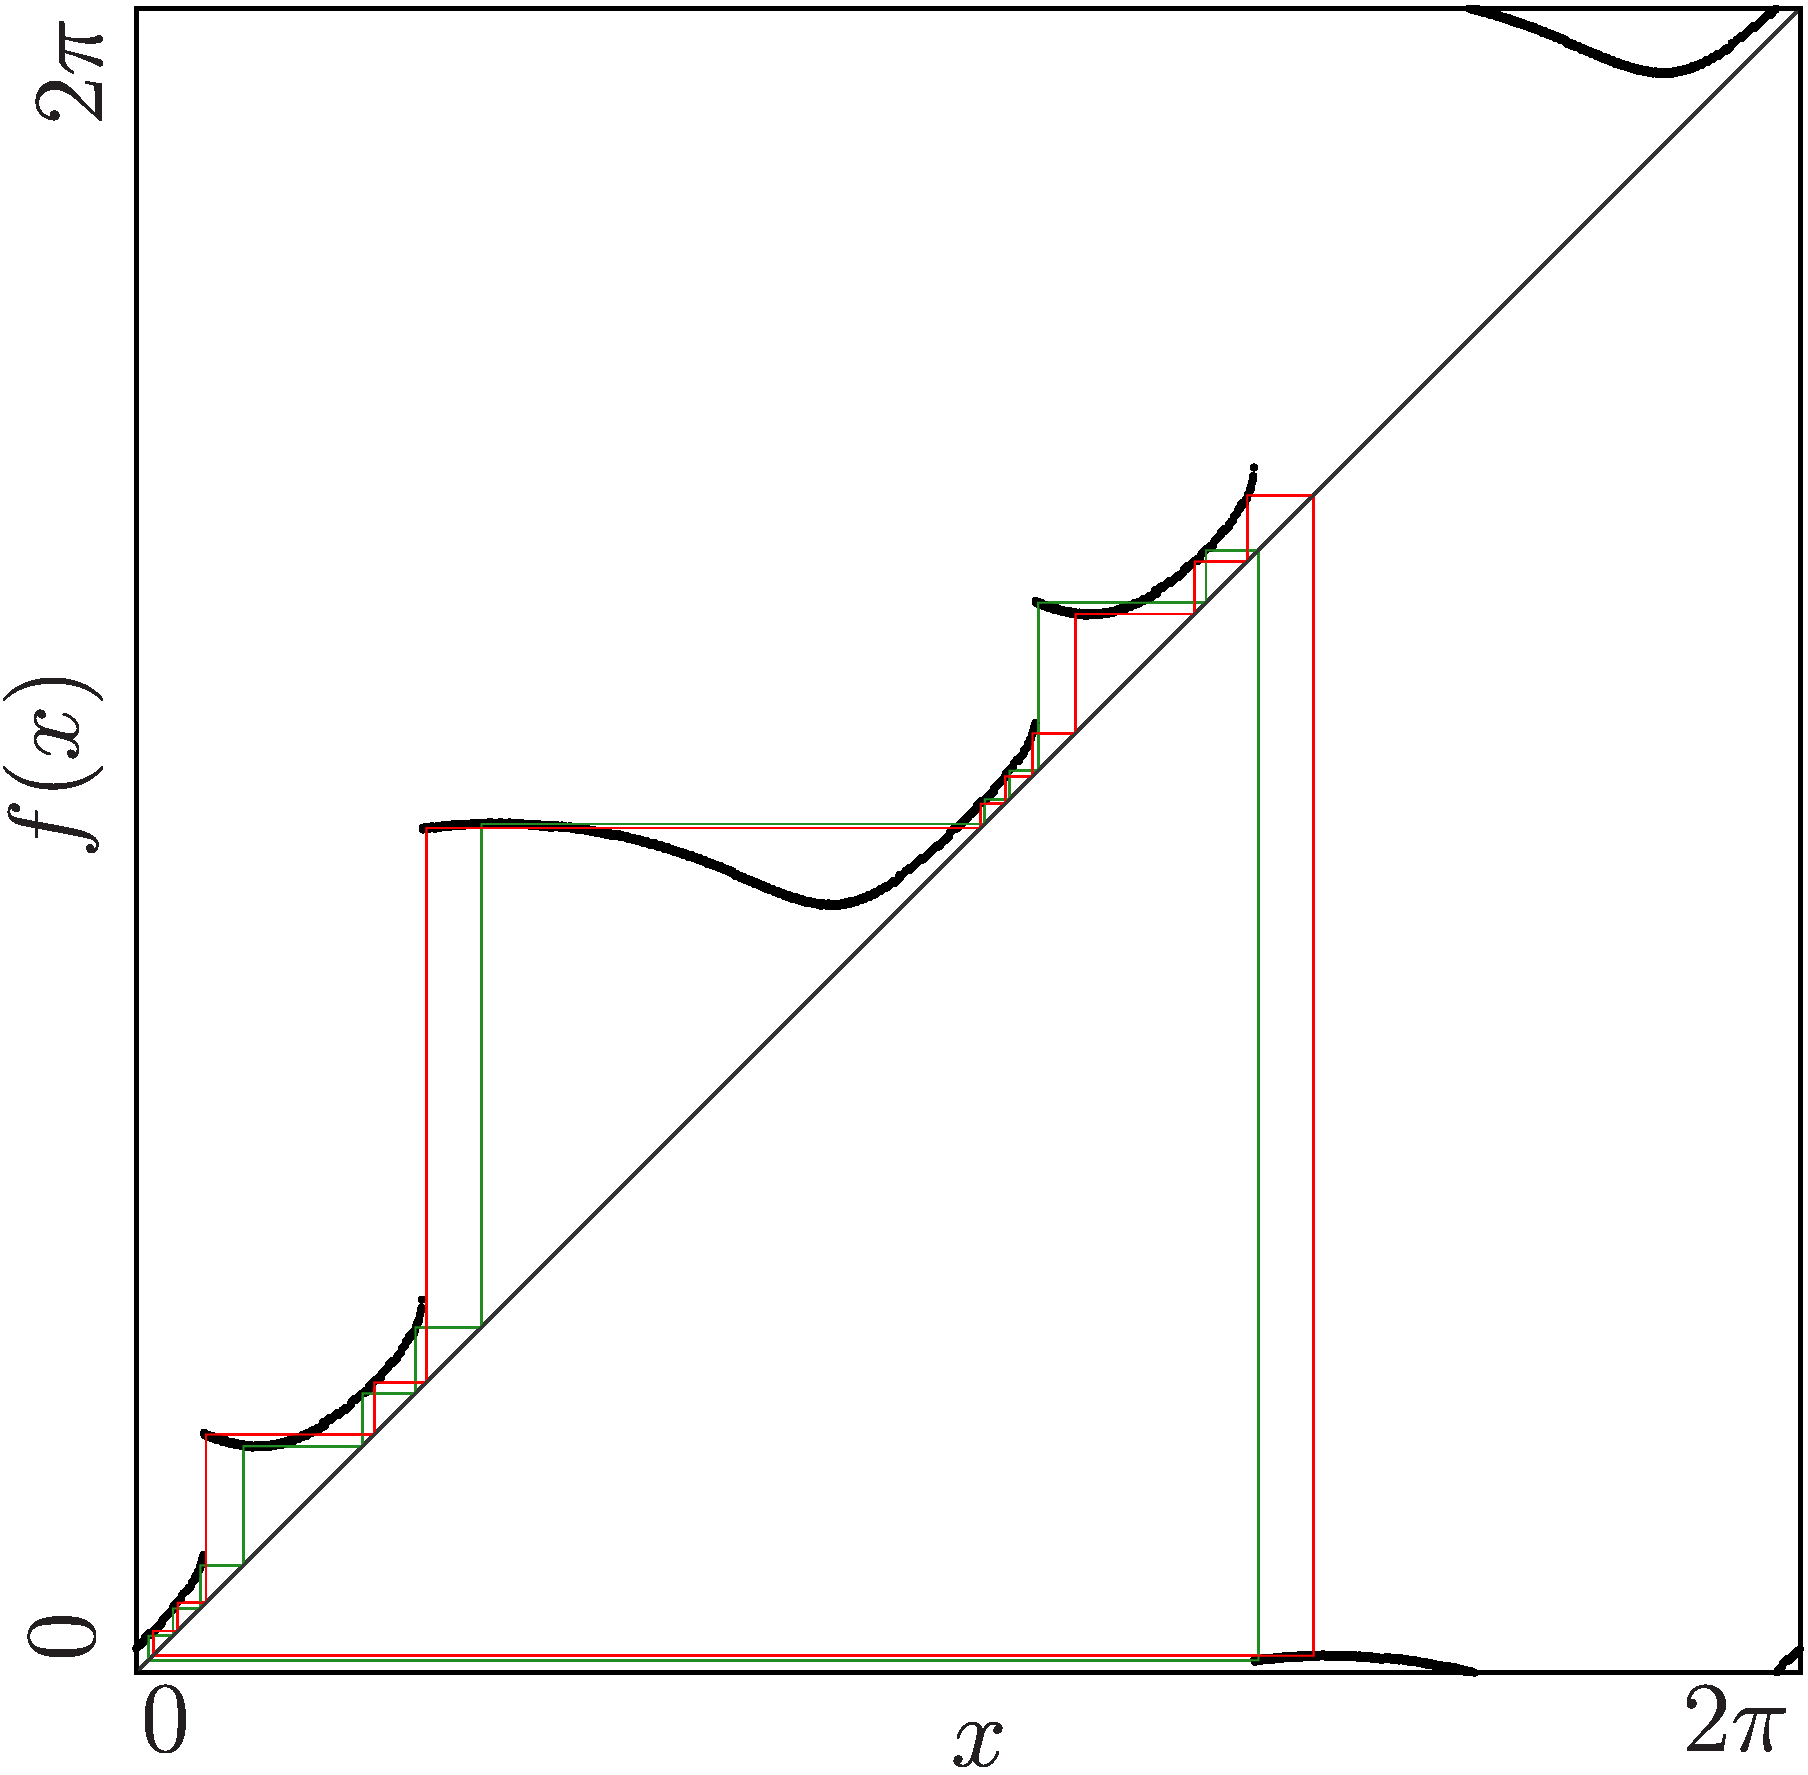
\includegraphics[width=0.3 \textwidth]{Figs/og_model_cycle_b.png}
			}{$B:\:\A^3\B^3\C^2\D^4,\:\A^2\B^4\C^3\D^3$}
			\stackunder[5pt]{
				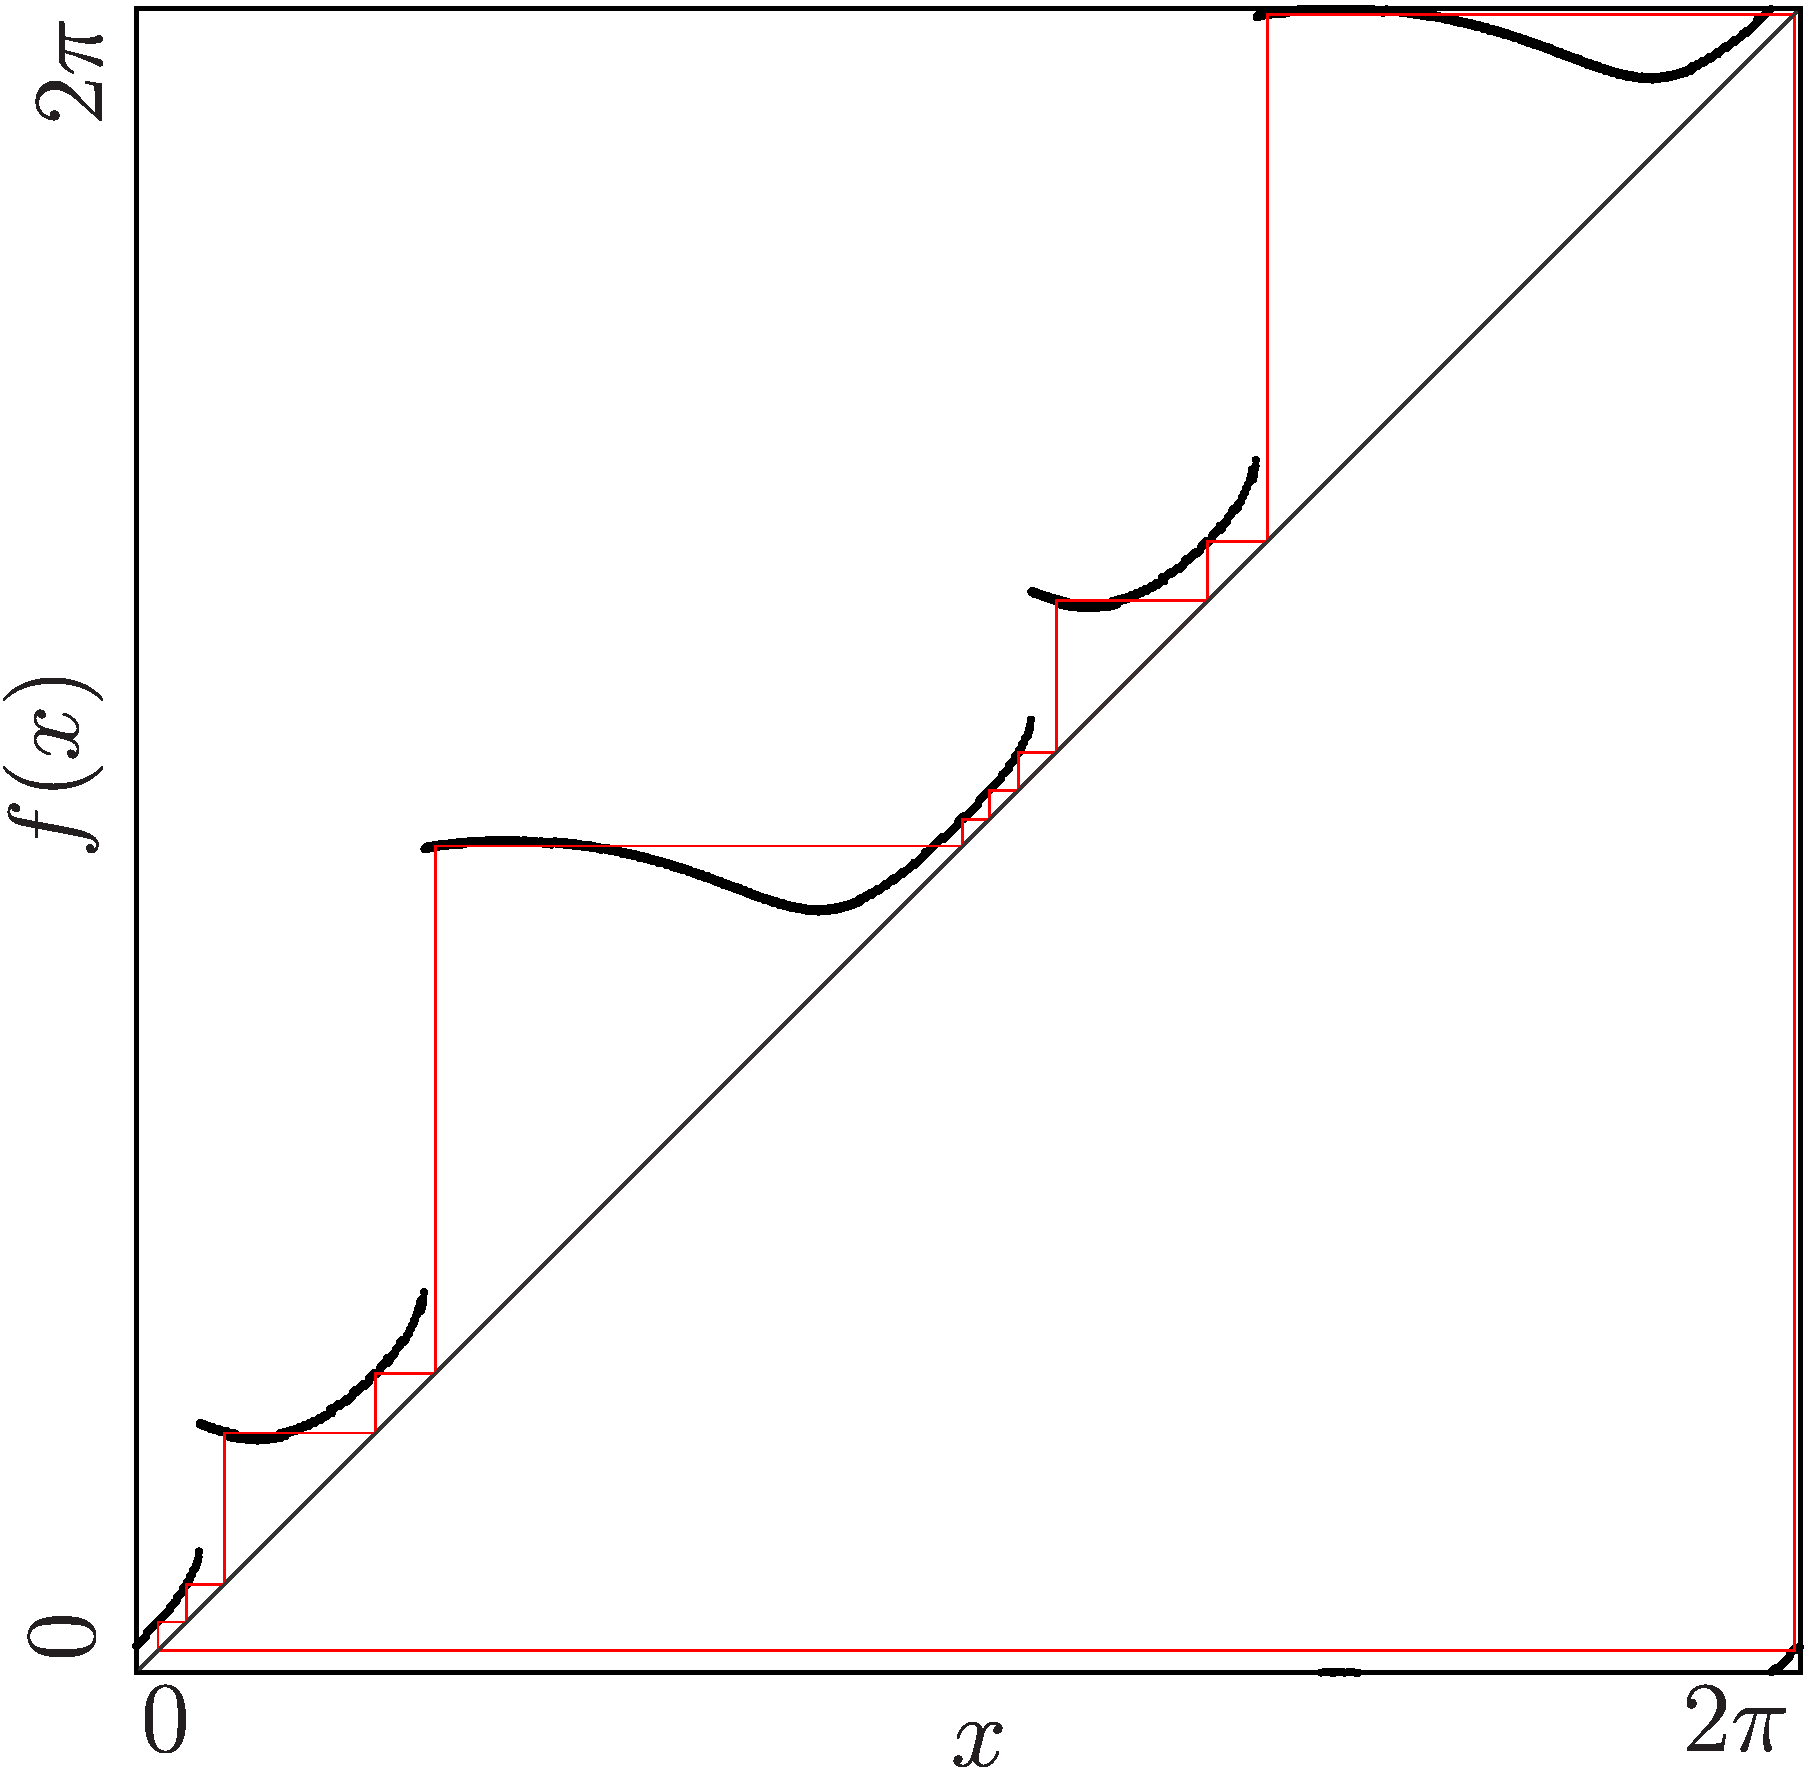
\includegraphics[width=0.3 \textwidth]{Figs/og_model_cycle_c.png}
			}{$C:\:\A^2\B^4\C^2\D^4$}
		\end{figure}

		\vspace{1em}
		Symmetry $F(\theta + \pi) = F(\theta) + \pi \mod 2\pi$ \hfill [Akyuz] %\cite{akyuz2022}
	}
\end{frame}

%%% Local Variables:
%%% mode: latex
%%% TeX-master: "../Vortrag_Frauenhofer_Weik"
%%% End:
